\documentclass[a4paper,12pt]{article}

\usepackage{cmap}		
\usepackage[utf8]{inputenc}			
\usepackage[english,russian]{babel}
\usepackage{framed}
\usepackage{hyperref}
\usepackage{amsmath}
\usepackage[colorinlistoftodos]{todonotes}
\usepackage{wrapfig}
\usepackage{lipsum}
\usepackage{listings}
\usepackage{color}
\usepackage{indentfirst}
\usepackage{times}
\usepackage{textcomp}
\usepackage{smartdiagram}
\usepackage{caption}
\usesmartdiagramlibrary{additions}
\usepackage{tikz}
\usepackage{multicol}
\usepackage{lipsum}
\usepackage{mwe}
\usepackage{floatrow}
\usepackage[ruled]{algorithm2e}
\usepackage{subfigure}
\usepackage{subcaption}
\usepackage{minted}
\usepackage{placeins}
\usepackage{amsfonts}
\usepackage{subcaption}
\usepackage[T1]{fontenc}
\usepackage{tgbonum}
\usetikzlibrary{arrows,shapes}
\DeclareMathOperator*{\argmin}{arg\,min}
\DeclareMathOperator*{\argmax}{arg\,max}
\DeclareMathOperator{\E}{\mathbb{E}}
\definecolor{mygray}{rgb}{0.4,0.4,0.4}
\definecolor{mygreen}{rgb}{0,0.8,0.6}
\definecolor{myorange}{rgb}{1.0,0.4,0}

\lstdefinestyle{customc}{
  belowcaptionskip=1\baselineskip,
  breaklines=true,
  frame=L,
  xleftmargin=\parindent,
  language=C,
  showstringspaces=false,
  basicstyle=\footnotesize\ttfamily,
  keywordstyle=\bfseries\color{green!40!black},
  commentstyle=\itshape\color{purple!40!black},
  identifierstyle=\color{blue},
  stringstyle=\color{orange},
  numbers=left,
  numbersep=12pt,
  numberstyle=\small\color{mygray},
}
\lstset{escapechar=@,style=customc}


\newcommand{\HRule}{\rule{\linewidth}{0.5mm}}

\newcommand{\grayhl}[1]{{\fontfamily{cmss}\selectfont  \colorbox{gray!30}{>> #1}}}
\newcommand{\indgrayhl}[1]{{\fontfamily{cmss}\selectfont  \colorbox{gray!30}{\hspace{2.5cm} #1}}}

\begin{document}

\begin{titlepage}
\begin{center}

\textsc{\Large Московский Государственный Технический Университет имени Н.Э.Баумана}\\
\textsc{\large (Национальный Исследовательский Университет)}\\[1.5cm]

% Upper part of the page. The '~' is needed because \\
% only works if a paragraph has started.

\includegraphics[width=0.3\textwidth]{img/logo.png}~\\[1cm]

\textsc{\Large Отчёт по \\ Производственная Практика (Научно-исследовательская Практика) }\\[0.5cm]

% Title
\HRule \\[0.4cm]
{ \LARGE \bfseries Simultaneous localization and mapping (SLAM) \\[0.4cm] }

\HRule \\[1.5cm]

% Author and supervisor
\noindent
\begin{minipage}{0.4\textwidth}
\begin{flushleft} \large
\emph{Студент:}\\
Юнес \textsc{А.~Ю.}
\end{flushleft}
\end{minipage}%
\begin{minipage}{0.4\textwidth}
\begin{flushright} \large
\emph{Преподаватель:} \\
Ющенко \textsc{А.~С.}
\end{flushright}
\end{minipage}

\vfill

% Bottom of the page
{\large \today}

\end{center}
\end{titlepage}


\newpage
\tableofcontents

\newpage
\listoffigures

\newpage
\section{Introduction}

SLAM (Simultaneous localization and mapping) is the computational problem of constructing or updating a map of an unknown environment while simultaneously keeping track of an agent's location within it.

In Robotics, SLAM is necessary when:
\begin{enumerate}
    \item The robot must be truly work autonomously (without human inputs).
    \item We don't have a prior knowledge about the environment.
    \item We can't rely exclusively on pre-placed beacons or external positioning systems (e.g. GPS).
    \item The robot needs to know it is.
\end{enumerate}

To address SLAM problem, we have to divide it into its two core components; localization and mapping.\\
Localization problem is the backbone of spatial awareness of a robot, which is one of the most challenging problems in probabilistic robotics. The original (pure) localization problem needs a known map (which we don't have in the SLAM problem). In the other hand, Mapping problem concerns building a map of the environment, for which accurate pose estimation (accurate localization) is necessary. Simultaneously we have to estimate robot poses along the way, when we don't have a prior knowledge of the robot's workspace to solve the SLAM problem.
\begin{figure}[H]
    \centering
    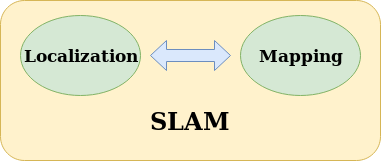
\includegraphics[width=\textwidth]{img/slam.png}
    \caption{Simultaneous Localization And Mapping (SLAM)}
    \label{fig:slam}
\end{figure}

\newpage
\section{Problem formulation}
The goal of this work, is to present the work done during the ETHz robotics summer school \cite{1}, which is related to localize and building the map for a mobile robot in uncertain conditions.\\
The SuperMegaBot (fig. \ref{fig:smb}) was used in the tutorials.
\begin{figure}[H]
    \centering
    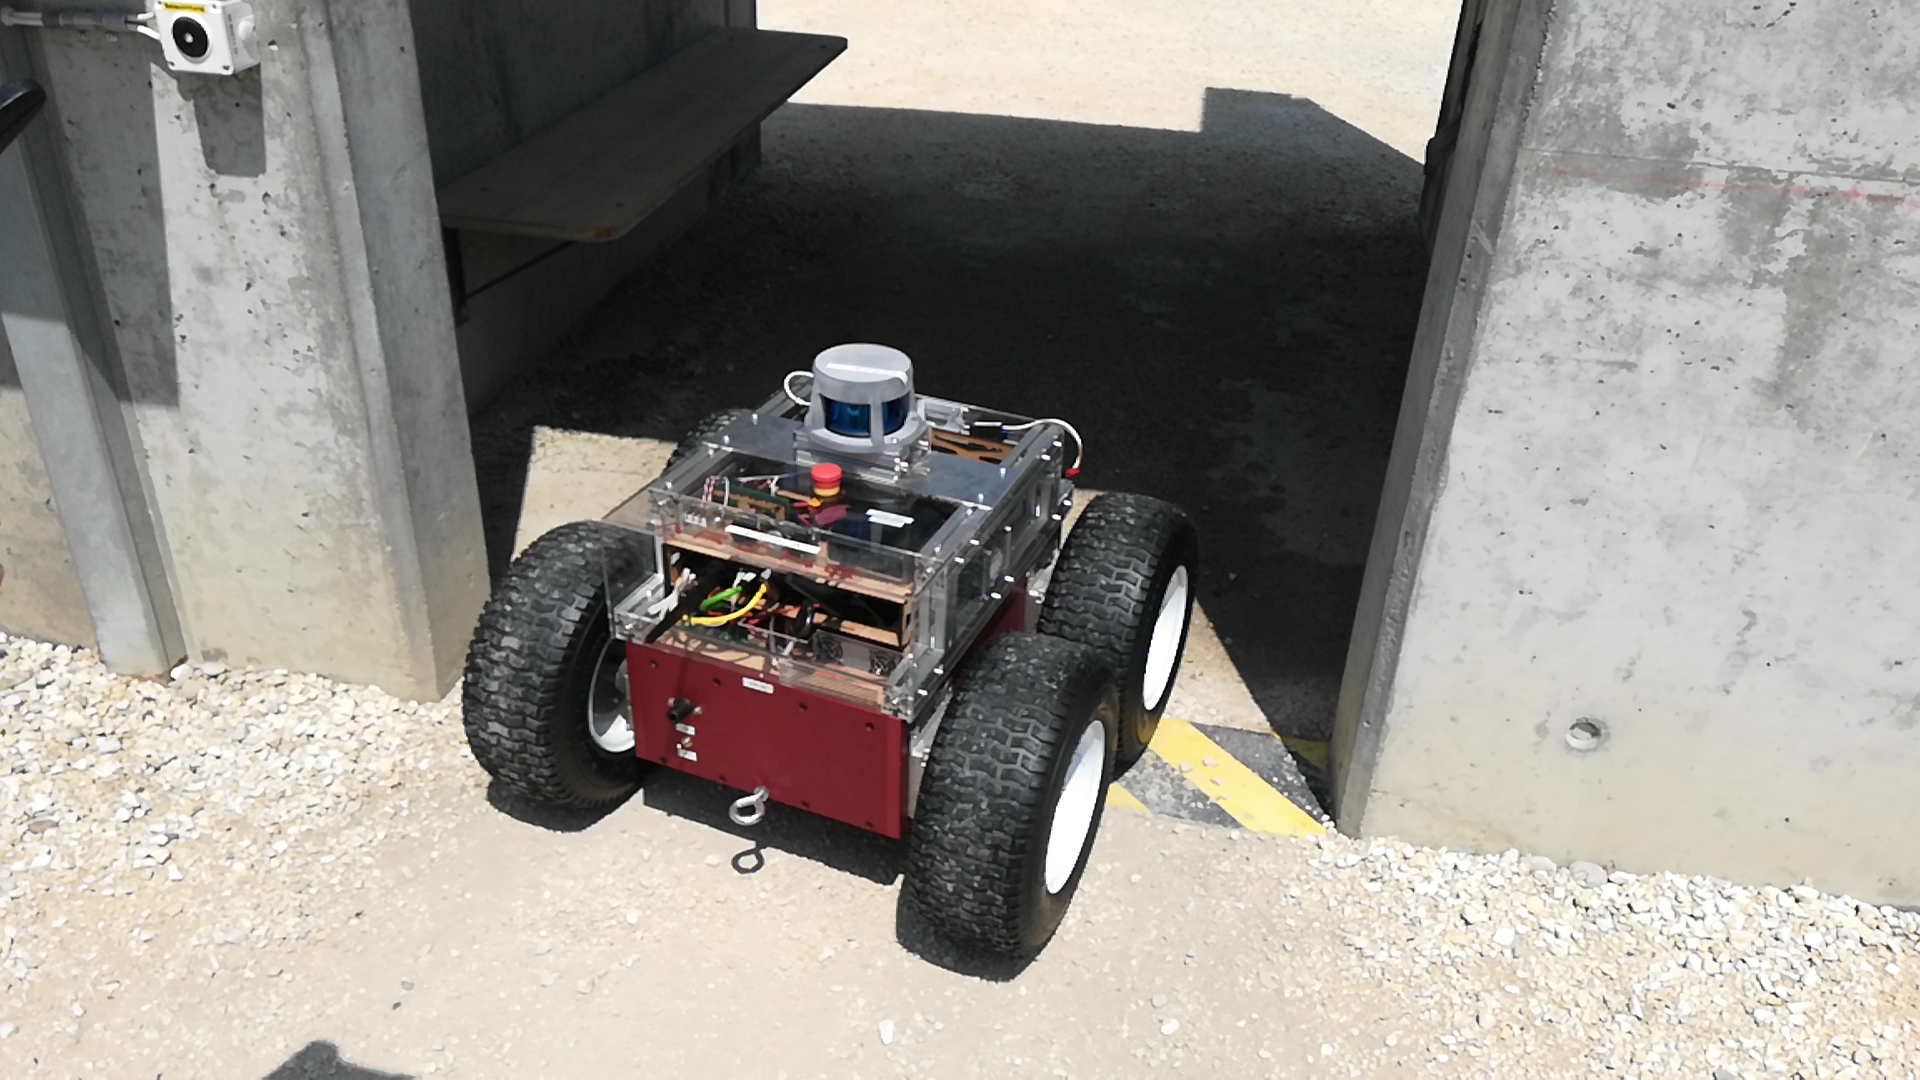
\includegraphics[width=\textwidth]{img/smb.jpg}
    \caption{The robot : SuperMegaBot}
    \label{fig:smb}
\end{figure}
To achieve that, we had to do the following:
\begin{enumerate}
\item Localization : \\
    Estimating the 6D position of the robot in the environment (state estimation); the dimensions are x,y,z and roll,pitch,yaw.\\
    The state estimator uses wheels' odometry, IMU (Inertial Measurement Unit) as the process measurements, and uses LIDAR to update measurements.\\
    We have used ConFusion \cite{2}- an open-source package, which was developed by the hosted laboratory.\\
    \begin{figure}[H]
    \centering
    
\includegraphics[width=\textwidth]{img/confusion.png}
    \caption{confusion}
    \label{fig:confusion}
    \end{figure}
\item Mapping :\\
    Build a map using the state estimator and sensory data; map representation will be : point cloud, grid, mesh ...\\
    the algorithm which is used to build the map, is called Iterative Closest Point (ICP), avilable as a ROS-package (ethzasl icp mapping \cite{3}).
\end{enumerate}

\section{Theoretical Background} 
\subsection{The state estimator}
The state, is the minimal representation of the quantities to describe the robot's situation at any instant of time.\\
In robotics applications, we depend on the current state of the robot to move it to desired state, by sending the corresponding commands for that. The aforementioned paradigm can be shown as a closed-loop control system (fig. \ref{fig:control}), we need the state estimator to find a state correction, avoiding the effects of disturbances (and uncertainties) on the robot.

\begin{figure}[H]
\centering
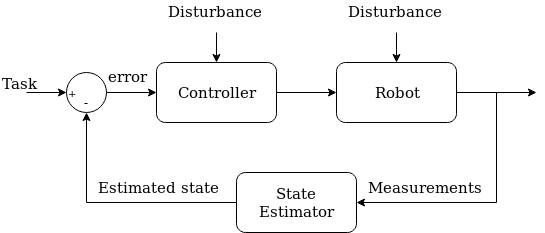
\includegraphics[width=\textwidth]{img/control(1).png}
\caption{A closed-loop control system}
\label{fig:control}
\end{figure}

The state estimator should use the Sensors and measurements models to obtain the next state; In this models we have two types:
\begin{enumerate}
    \item Process Measurement ($\hat{p_t}$): a model provides information about the change in the robot state from one instance to the next;
    $$x_{t+j}=h(x_t,\hat{p_{t:t+j}},s)$$
    This model get its data from the motion prior, IMU, joint torque sensors and wheel speed sensors
    \item Update Measurement ($\hat{u_t}$): provides information about the robot state at a discrete time instances;
    $$\hat{u_t}=g(x_t,s)$$
    For example data from Camera, LIDAR, and joint encoders.
\end{enumerate}
 The available sensors in supermegabot are shown in fig. \ref{fig:smb_sensors}
\begin{figure}[H]
\centering
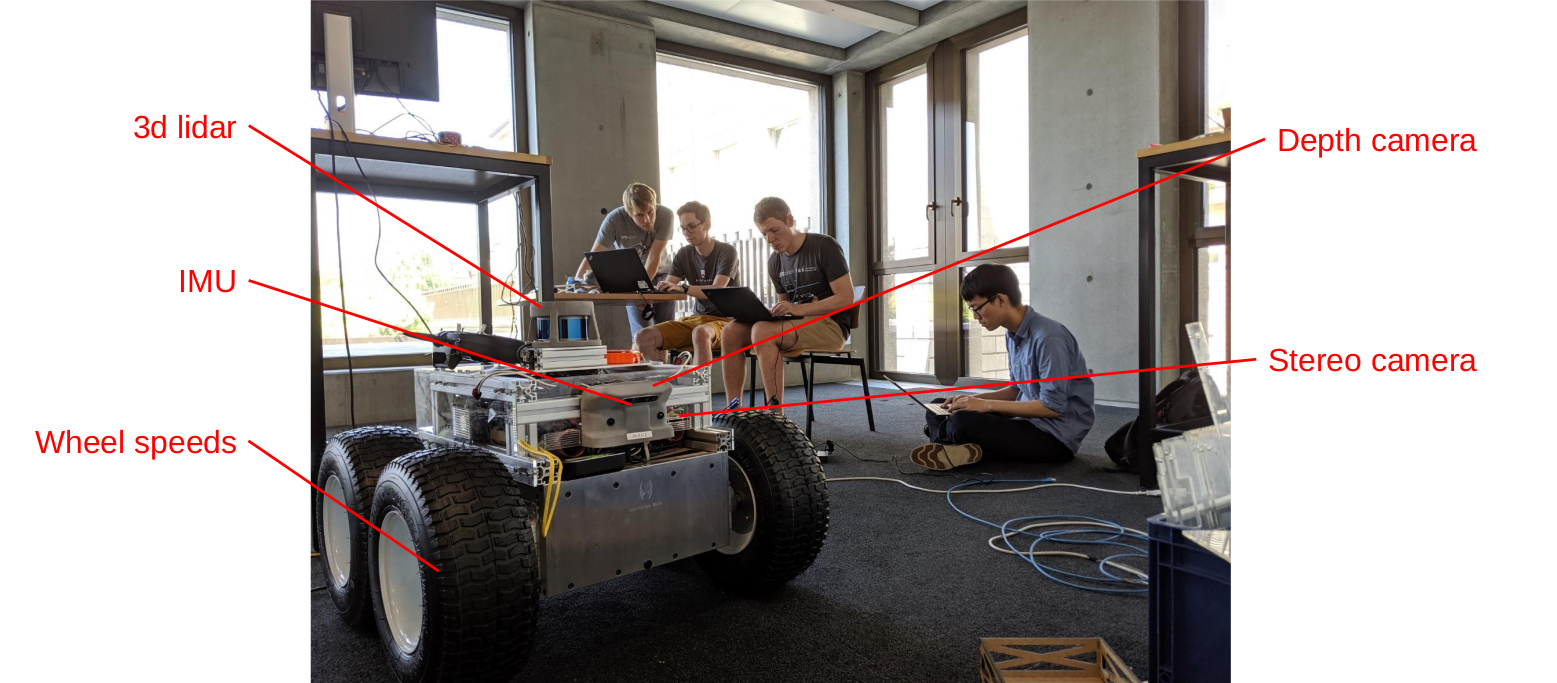
\includegraphics[width=\textwidth]{img/smb_sensors.png}
\caption{Supermegabot sensors}
\label{fig:smb_sensors}
\end{figure}

We can see the structure of the state estimation problem like in the diagram (fig \ref{fig:dia1})
\begin{figure}[H]
\centering
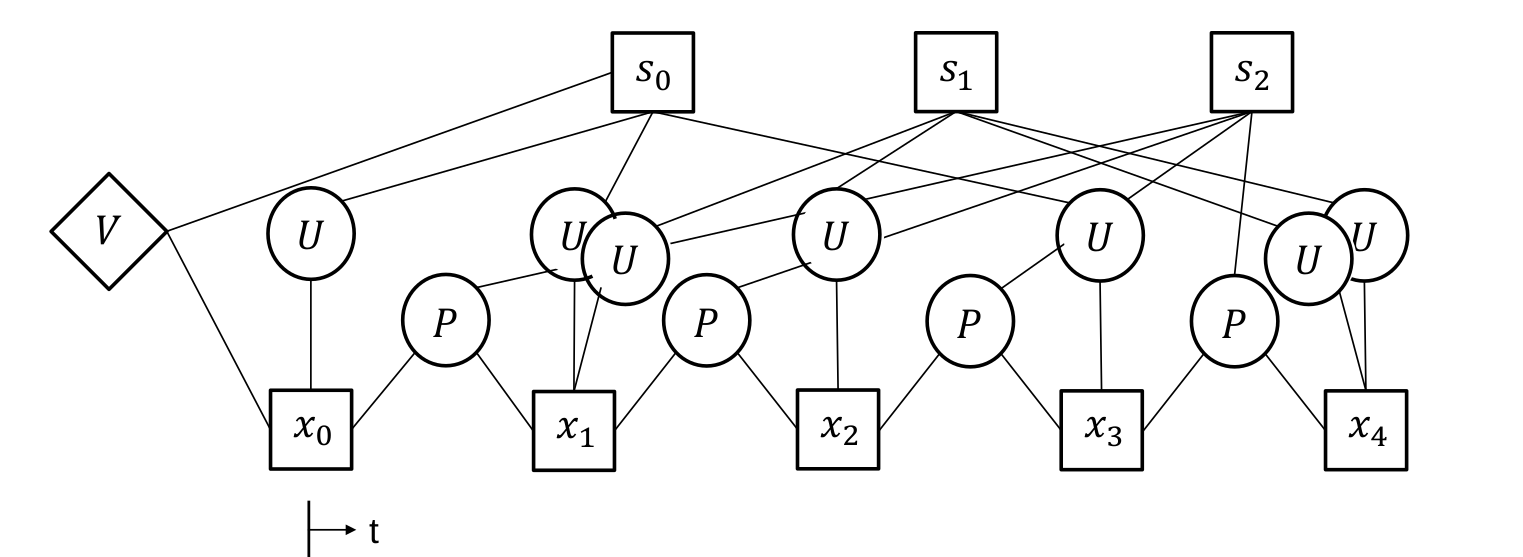
\includegraphics[width=\textwidth]{img/dia1.png}
\caption{State estimation diagram}
\label{fig:dia1}
\end{figure}

Where V stands for the prior knowledge (initial guess) about the robot position, U the update measurements (LIDAR in our case), P Process Measurements (odometry and IMU) , while x and s are the states.

We want to find the set of the robot states which are best described by measurements; if we consider a series of N time-steps (a window), we can formulate it by the following optimization problem: 
$${x*_{t_0,t_N},s*}=\argmax_{x_0,N,s}p(x_{t_0,t_N},s|U,P,V)$$
or after factorization:
$${x*_{t_0,t_N},s*}=\argmax_{x_0,N,s}\left[ p(x_0,s|V) \prod_{i=0}^N \left(\prod_{\hat{u}\in U} p(\hat{u}|x_i,s)\right) \prod_{i=0}^N \left(\prod_{\hat{p}\in P} p(x_i|x_{i-1},s,\hat{p}^{i-1:i})\right) \right]$$
If we consider well-behaved models and normally distributed noise; we can work to minimize the errors:
$${x*_{t_0,t_N},s*}=\argmin_{x_0,N,s}\left[ e_v(x_0,s,V) \sum_{i=0}^N \left(\sum_{\hat{u}\in U} e_u(x_i,s,\hat{u})\right) \sum_{i=0}^N \left(\sum_{\hat{p}\in P} e_p(x_{i-1},x_i,s,\hat{p}^{i-1:i})\right) \right]$$
Assuming an initial guess on selected parameters with some normally distributed confidence; the equation could be written:
$${x*_{t_0,t_N},s*}=\argmin_{x_0,N,s}\left[ \begin{split}
\left|\left|\begin{matrix}\hat{x}_{t_0}-x_{t_0}\\ \hat{s} - s\end{matrix}\right|\right|^2_{W_M}+\sum^N_{i=0}\left(\sum_{\hat{u}\in U} ||\hat{u}-g(x_t,s)||^2_{W_{\hat{u}}}\right)\\+\sum^N_{i=0}\left(\sum_{\hat{p}\in P} ||x_{t_i}-h(x_{t_i-1},\hat{p},s)||^2_{W_{\hat{p}}}\right)
\end{split}
\right]$$
where $W_{\hat{u}}$ is the inverse of the covariance matrix in the units of sensor readings $W_{\hat{u}}=\sum^{-1}_{\hat{u}}$..

The result in a non-linear least squares optimization problem, we can get faster convergence by using methods like Levenberg-Marquart and Dogleg;
$$x*=\argmin_x \frac{1}{2}||f(x)||^2$$
$$\delta x*=\argmin_{\delta x}\frac{1}{2}||j(x)\delta x +f(x)||^2$$
$$J(x)^T J(x)\delta x*=-J(x)^T f(x)$$
$$H(x) \delta x*=b(x)$$
We can use sparse Cholesky solver to solve this problem effectively.
\newpage
To formulate this problem to work online, we can form a Moving Horizon Estimator, by choosing an appropriate N, and removing the desired parameters through Gaussian Elemenation on the system Hx=b.
Or marginalize measurements sequentially out of the problem and incorporate it into the estimated parameter distribution (V). This method called recursive filtering.

\begin{figure}[H]
\centering
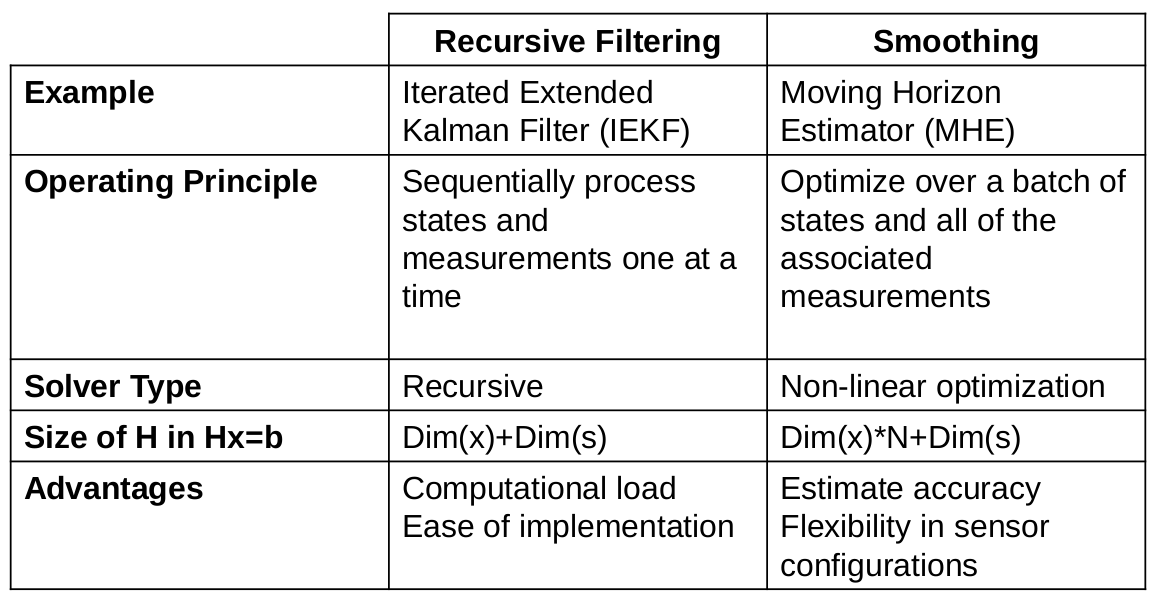
\includegraphics[width=\textwidth]{img/table.png}
\caption{Comparison table}
\label{fig:table}
\end{figure}

For supermegabot, we have used ConFusion \cite{2} (Sensor Fusion for Complex Robotic Systems using Nonlinear Optimization) ; which is a general framework for MHE operation, wraps around Ceres solver, allowing the usage of a wide range of non-linear solvers and auto-differentiation.
\begin{figure}[H]
\centering
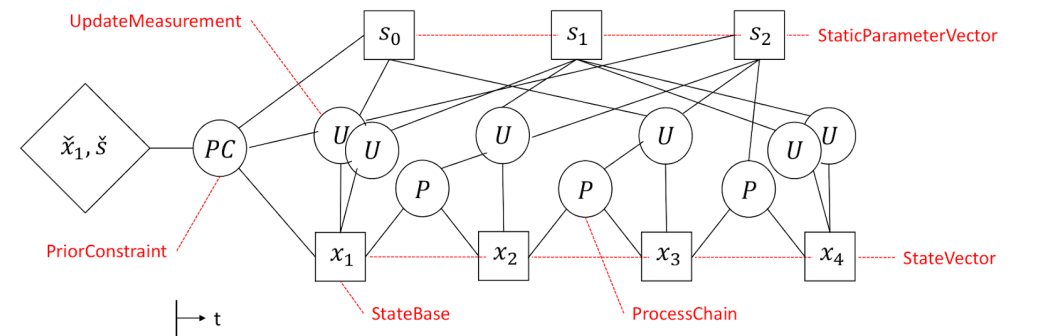
\includegraphics[width=\textwidth]{img/conf.png}
\caption{ConFusion diagram}
\label{fig:conf}
\end{figure}

\newpage
\subsection{ICP Mapper}
Iterative closest point (ICP) \cite{4} \cite{5} \cite{6} is an algorithm employed to minimize the difference between two clouds of points. ICP is often used to reconstruct 2D or 3D surfaces from different scans, to localize robots and achieve optimal path planning (especially when wheel odometry is unreliable due to slippery terrain).\\

The problem can be formulated by the following; given two corresponding point sets:
$$X = {x_1,...x_N}$$
$$P={p_1,...,p_N}$$
we want to find the transition t and the rotation R that minimize the sum of the squared errors:
$$E(R,t)=\frac{1}{N}\sum^{N_p}_{i=1}||x_i-Rp_i-t||^2$$
if the correct correspondences are known, the correct relative rotation/translation can be calculated in a closed form; by the following steps:
\begin{enumerate}
    \item Subtract the corresponding center of mass from every point in the two point sets; 
    $$X'={x_i-\mu_x}={x_i'},... \mu_x=\frac{1}{N}\sum^N_{i=1}x_i$$
    $$P'={p_i-\mu_p}={p_i'},... \mu_p=\frac{1}{N}\sum^N_{i=1}p_i$$
    \item Find the Singular Value Decomposition (SVD) of matrix W ; where $W=\sum^N_{i=1} x_i' p_i'^T$
    $$SVD(W): W=U\Sigma V$$
    $\Sigma$ is a diagonal matrix with singular values in it main diagonal
    \item \textbf{Theorem} : if rank(W)=3, the optimal solution of E(R,T) is unique and is given by:
    $$R=UV^T$$
    $$t=\mu_x-R\mu_p$$
    and the minimal value of the error function at (R,T) is:
    $$E(R,T)=\sum^N_{i=1}(||x_i'||^2+||y_i'||^2)-2(trace(\Sigma))$$
    where $trace(\Sigma)$ = the sum of elements of the main diagonal.
\end{enumerate}

If the correct correspondences are not known, it is impossible to determine the optimal relative rotation and translation in one step. here came the idea of ICP; iterate to find alignment.\\

ICP has the following variants:
\begin{enumerate}
    \item Point subsets (from one or both point subsets).
    \item Weighting the correspondences.
    \item Data association.
    \item Rejecting outlier point pairs.
\end{enumerate}
The ICP algorithm consists of the following steps:
\begin{enumerate}
    \item Potentially sample points.
    \item Determine corresponding points.
    \item Potentially weight/reject pairs.
    \item Compute rotation R, translation t (e.g. SVD).
    \item Apply R and t to all points of the set to be registered.
    \item Compute the error E(R,t)
    \item if error decreased but still bigger than a threshold; then repeat to determine correspondences, until you reach the point where the error less than the threshold; stop and output the final alignment.
\end{enumerate}
\newpage
Default Configuration of the ICP Chain\footnote{https://github.com/ethz-asl/libpointmatcher/blob/master/doc/DefaultICPConfig.md}
\begin{figure}[H]
\centering
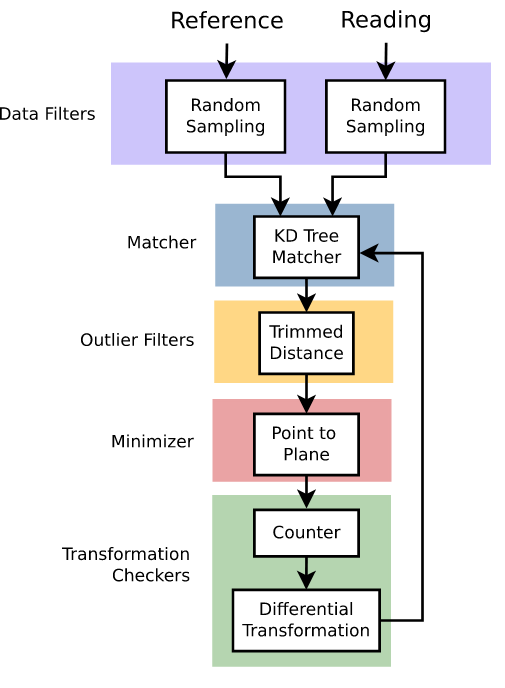
\includegraphics[width=0.6\textwidth]{img/icp_chain.png}
\caption{Default ICP chain configuration}
\label{fig:icp}
\end{figure}
\begin{itemize}
    \item Data Filters:\\
Both the reference and reading clouds are processed with random sampling filters. These will sample each data point with a probability of 0.75 thus yielding smaller point clouds.
\item Matcher:\\
The default matcher is the KD tree matcher. Each point is matched to its closest neighbor in the reference cloud. A KD tree with a linear heap is used.

\item Outlier Filters\\
One trimmed distance outlier filter is used. The filter ranks the points in the reading cloud by their distance to the reference after a transformation was applied. The top 85\% points (those with the smallest distances) are kept.

\item Minimizer:\\
The point-to-plane variant is used in the minimization step. Point-to-plane allows for points to "slide" along planes and generally performs better than the point-to-point variant.

\item Transformation Checkers:\\
The counter checker automatically stops the ICP loop after a maximum of 40 iterations. The differential transformation checker stops the ICP loop when the relative transformation motions between iterations is below a threshold. In other words, when each subsequent iteration produces little change in the transformation, then the algorithm is stopped. Because the relative motions are generally prone to jagged oscillations, smoothing is applied by taking the average the relative differences over several iterations.
\end{itemize}
\newpage
\section{Experimental part}
The goals of the experimental part is :
\begin{tighitemize}
    \item Run the state estimator (Confusion algorithm).
    \item Run the ICP based mapper.
    \item Save and load point cloud maps.
\end{tighitemize}

Steps to prepare your PC to work with the robot:\\
(The following steps tested on \textbf{ubuntu 18.04} and \textbf{ROS melodic}.)
\begin{enumerate}
    \item install the following dependencies:\\
    {\fontfamily{cmss}\selectfont \colorbox{gray!30}{>> sudo apt update }}\\
{\fontfamily{cmss}\selectfont  \colorbox{gray!30}{>> sudo apt-get install git python-catkin-tools doxygen}}\\
{\fontfamily{cmss}\selectfont  \colorbox{gray!30}{>> sudo apt-get install ros-melodic-octomap ros-melodic-octomap-msgs \textbackslash }}\\ 
{\fontfamily{cmss}\selectfont  \colorbox{gray!30}{\hspace{2.5cm}  ros-melodic-octomap-ros ros-melodic-rosserial ros-melodic-joy \textbackslash}}\\
{\fontfamily{cmss}\selectfont  \colorbox{gray!30}{\hspace{2.5cm}ros-melodic-ompl ros-melodic-costmap-2d \textbackslash}}\\ {\fontfamily{cmss}\selectfont  \colorbox{gray!30}{\hspace{2.5cm}ros-melodic-velodyne-gazebo-plugins}}\\
{\fontfamily{cmss}\selectfont  \colorbox{gray!30}{>> sudo apt-get install libpcap0.8-dev libeigen3-dev libopencv-dev libboost-dev \textbackslash}}
{\fontfamily{cmss}\selectfont  \colorbox{gray!30}{\hspace{2.5cm}ros-melodic-cmake-modules libssh2-1-dev}}\\
{\fontfamily{cmss}\selectfont  \colorbox{gray!30}{>> sudo apt-get install libglpk-dev python-wstool net-tools}}\\
{\fontfamily{cmss}\selectfont  \colorbox{gray!30}{>> sudo apt-get install liblapack-dev libblas-dev autotools-dev dh-autoreconf \textbackslash}} \\
{\fontfamily{cmss}\selectfont  \colorbox{gray!30}{\hspace{2.5cm}libboost-all-dev python-setuptools cppcheck default-jre libgtest-dev \textbackslash}}\ \\
{\fontfamily{cmss}\selectfont  \colorbox{gray!30}{\hspace{2.5cm}libglew-dev clang-format-3.9 python-git pylint python-termcolor\textbackslash}} \\
{\fontfamily{cmss}\selectfont  \colorbox{gray!30}{\hspace{2.5cm} "ros-melodic-camera-info-manager*" protobuf-compiler \textbackslash}} \\
{\fontfamily{cmss}\selectfont  \colorbox{gray!30}{\hspace{2.5cm} protobuf-c-compiler libssh2-1-dev libatlas3-base libnlopt-dev \textbackslash}} \\
{\fontfamily{cmss}\selectfont  \colorbox{gray!30}{\hspace{2.5cm}"ros-melodic-tf2-*" python-pip python-autopep8 libreadline-dev ifstat\textbackslash}} \\ 
{\fontfamily{cmss}\selectfont  \colorbox{gray!30}{\hspace{2.5cm} ntpdate sysstat libv4l-0 ros-melodic-gps-common \textbackslash}}

    \item Create and setup the catkin workspace:\\
    \grayhl{mkdir -p ~/catkin\_ws/src}\\
    \grayhl{cd ~/catkin\_ws}\\
\grayhl{catkin init}\\
\grayhl{catkin config --extend /opt/ros/melodic}\\
\grayhl{catkin config --merge-devel}\\
\grayhl{catkin config -DCMAKE\_BUILD\_TYPE=Release}\\

\item Clone the repisotory Use wstool to manage external packages in the workspace:\\
\grayhl{cd ~/catkin\_ws/src/}\\
\grayhl{git clone https://github.com/ethz-asl/eth\_supermegabot.git}\\
\grayhl{wstool init}\\
\grayhl{wstool merge eth\_supermegabot/dependencies.rosinstall}\\
\grayhl{wstool up}

    \item Build the workspace (it will take time):\\
\grayhl{cd ~/catkin\_ws/}\\
\grayhl{catkin build}
    
    \item Source the workspace:\\
\grayhl{source devel/setup.bash}\\
    you can add the workspace to the ~/.bashrc file, so it will be sourced every time you run the terminal:\\
\grayhl{echo "source ~/catkin\_ws/devel/setup.bash" >> ~/.bashrc}
    
\end{enumerate}

You have to do the previous steps just one time, after that:
\begin{enumerate}
    \item Check whether you have the latest version nad build:\\
    \grayhl{cd ~/catkin\_ws/src/eth\_supermegabot}\\
    \grayhl{git pull}\\
    \grayhl{wstool up}\\
    \grayhl{catkin build map\_interface}\\
    \grayhl{catkin build ethzasl\_icp\_mapper}\\
    \grayhl{catkin build smb\_state\_estimator}
    \item Change the configuration of the state estimator to use IMU, Odometry and LIDAR;\\
    \grayhl{roscd smb\_confuser}\\
    \grayhl{gedit config/smb\_calibration.cfg}\\
    and change it to the following:\\
    \indgrayhl{forwardPropagationSensor 0}\\
\indgrayhl{useImu true}\\
\indgrayhl{useBmm true}\\
\indgrayhl{useTags false}\\
\indgrayhl{useLidar true}

    \item Run the ICP mapper (on a bag file \footnote{\href{https://drive.google.com/drive/u/0/folders/1foJMIb1gbzVcuLtjc4Cu6ztEUZlDsP2W}{link to bag files}}):
    you need to run the following in seperate terminals:\\
    Terminal 1: \\ \grayhl{roscore}\\
    Terminal 2:\\ \grayhl{rosparam set use\_sim\_time true}\\
     \grayhl{robag play --clock slam.bag}\\
    Terminal 3:\\ \grayhl{roslaunch smb\_state\_estimator smb\_state\_estimator\_standalone.launch}
    Terminal 4:\\ \grayhl{roslaunch ethzasl\_icp\_mapper
supermegabot\_dynamic\_mapper.launch}
    Terminal 5:\\ \grayhl{rosrun rviz rviz -d rviz/slam.rviz}
    
    \item Now you can see forming the map in rviz;
    \begin{figure}[H]
        \centering
        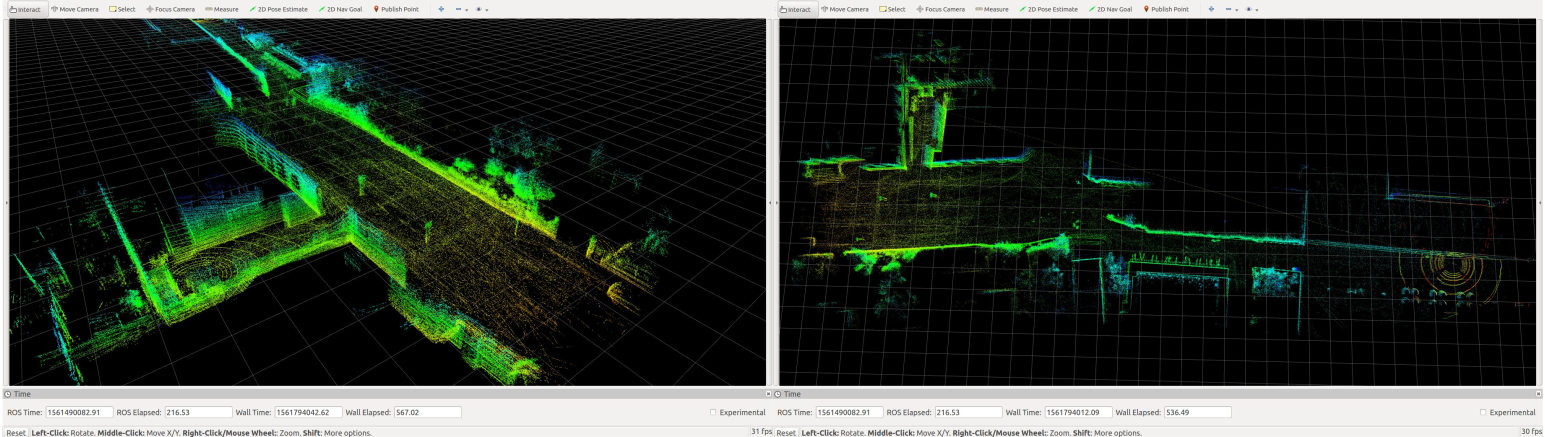
\includegraphics[width=\textwidth]{img/rviz1.png}
        \caption{ICP mapper in action}
        \label{fig:rviz1}
    \end{figure}
    \item To save the current map, you can use a ros service:\\
    \grayhl{rosservice call /mapper/save\_map "filename: data: '/home/ XXX/final\_map'" }\\
    you will need just the generated final\_map.pcd.
\end{enumerate}
\newpage
To load the previous map before running a second mission, you have to:
\begin{enumerate}
    \item Set your map file to be used by "map\_interface" package;\\
    \grayhl{roscd map\_interface/launch}\\
    \grayhl{gedit map\_interface.launch}\\
    Change the argument to mention your saved map;\\
    {\fontfamily{cmss}\selectfont  \colorbox{gray!30}{<arg name="map\_file" default="/home/ XXX/final\_map.pcd" />}}
    \item Run the following in separate terminals:\\
    Terminal 1: \\ \grayhl{roscore}\\
    Terminal 2:\\ \grayhl{rosparam set use\_sim\_time true}\\
     \grayhl{robag play --clock slam2.bag}\\
    Terminal 3:\\ \grayhl{roslaunch smb\_state\_estimator smb\_state\_estimator\_standalone.launch}
    Terminal 4:\\ \grayhl{roslaunch ethzasl\_icp\_mapper
supermegabot\_dynamic\_mapper.launch}
    Terminal 5:\\ \grayhl{roslaunch map\_interface map\_interface.launch}\\
    Terminal 6:\\ \grayhl{rosrun rviz rviz -d rviz/slam.rviz}
    \item Switch to rviz; right click on the marker (fig. \ref{fig:rviz2}) ans select "Load map"
    \begin{figure}[H]
        \centering
        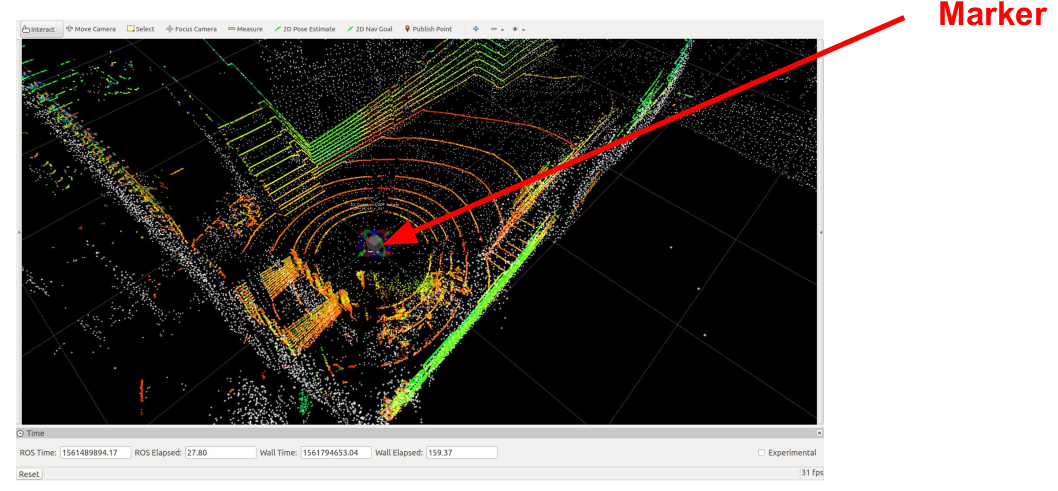
\includegraphics[width=\textwidth]{img/rviz2.png}
        \caption{Load a saved map - rviz}
        \label{fig:rviz2}
    \end{figure}
\end{enumerate}
\newpage
To run the experiment on the real robot; after following the instruction to connect to the robot \footnote{\href{https://drive.google.com/file/d/1zAdCP-8CdNpKgCalGuF-PEPpDxUV0_GZ/view}{link to the instructions }}; run this in separate terminals:\\
Terminal 1:\\
\grayhl{roscore}\\
Terminal 2:\\
LPC (state estimation and controllers)\\
\grayhl{roslaunch smb\_lpc lpc.launch}\\
Terminal 3:\\
\grayhl{roslaunch ethzasl\_icp\_mapper supermegabot\_robotsense\_dynamic\_mapper.launch}\\

On the Operating PC run:\\
\grayhl{roslaunch smb\_opc opc.launch}
\newpage
\begin{thebibliography}{9}
    \addcontentsline{toc}{section}{\refname}
    \bibitem{1} https://robotics-summerschool.ethz.ch/
\bibitem{2} Sandy, T., Stadelmann, L., Kerscher, S., Buchli, J. (2019). Confusion: Sensor fusion for complex robotic systems using nonlinear optimization. IEEE Robotics and Automation Letters, 4(2), 1093-1100.
\bibitem{3} https://wiki.ros.org/ethzasl\_icp\_mapping
\bibitem{3} Besl, P. J.,  McKay, N. D. (1992, April). Method for registration of 3-D shapes. In Sensor fusion IV: control paradigms and data structures (Vol. 1611, pp. 586-606). International Society for Optics and Photonics.
\bibitem{5} Pomerleau, F., Colas, F.,  Siegwart, R. (2015). A review of point cloud registration algorithms for mobile robotics. Foundations and Trends® in Robotics, 4(1), 1-104.
\bibitem{6} http://ais.informatik.uni-freiburg.de/teaching/ss16/robotics/slides/18-icp.pdf


\end{thebibliography}

\end{document}

\usepackage[english,russian]{babel}